\documentclass[conference]{IEEEtran}
\IEEEoverridecommandlockouts
% The preceding line is only needed to identify funding in the first footnote. If that is unneeded, please comment it out.
\usepackage{cite}
\usepackage{amsmath,amssymb,amsfonts}
\usepackage{algorithmic}
\usepackage{graphicx}
\usepackage{textcomp}
\usepackage{xcolor}
\usepackage{multicol}
\usepackage{float}
\def\BibTeX{{\rm B\kern-.05em{\sc i\kern-.025em b}\kern-.08em
    T\kern-.1667em\lower.7ex\hbox{E}\kern-.125emX}}
    
\usepackage[utf8]{inputenc}

\usepackage{listings}
\usepackage{xcolor}

%New colors defined below
\definecolor{codegreen}{rgb}{0,0.6,0}
\definecolor{codegray}{rgb}{0.5,0.5,0.5}
\definecolor{codepurple}{rgb}{0.58,0,0.82}
\definecolor{backcolour}{rgb}{0.95,0.95,0.92}

%Code listing style named "mystyle"
\lstdefinestyle{mystyle}{
  backgroundcolor=\color{backcolour},   commentstyle=\color{codegreen},
  keywordstyle=\color{magenta},
  numberstyle=\tiny\color{codegray},
  stringstyle=\color{codepurple},
  basicstyle=\ttfamily\footnotesize,
  breakatwhitespace=false,         
  breaklines=true,                 
  captionpos=b,                    
  keepspaces=true,                 
  numbers=left,                    
  numbersep=5pt,                  
  showspaces=false,                
  showstringspaces=false,
  showtabs=false,                  
  tabsize=2
}

%"mystyle" code listing set
\lstset{style=mystyle}

\date{ }

\pagenumbering{arabic}
    
\begin{document}

\begin{titlepage}
	\centering
        \vspace*{3cm}
		\includegraphics[width=9cm]{bangor_logo.pdf}
		
		\vspace*{1.5cm}            
        \huge
        \textbf{Laser-Based Free Space Communications}
           
        \vspace{2cm}
        \Large
        Murali Wood
        
        \Large
        Supervisor: Dr Roger Giddings
        \vfill
            

        \large
        School of Computer Science and Electronic Engineering\\
        College of Environmental Sciences and Engineering\\
        Bangor University\\
        \vspace*{0.8cm}
        \normalsize
        May 2021


\clearpage

\thispagestyle{empty} 
\centering
    \textbf Statement of Originality \\
    The work presented in this dissertation is entirely from the studies of the individual student, except where otherwise stated. Where derivations are presented and the origin of the work is either wholly or in part from other sources, then full reference is given to the original author. This work has not been presented previously for any degree, nor is it at present under consideration by any other degree awarding body. \\
    
    \centerline{\includegraphics[width=0.1\linewidth]{sig2.jpg}\par}
    
    Statement of Availability \\
    I hereby acknowledge the availability of any part of this dissertation for viewing, photocopying or incorporation into future studies, providing that full reference is given to the origins of any information contained herein.
    
    \centerline{\includegraphics[width=0.1\linewidth]{Sig2.jpg}\par}
    
\end{titlepage}

\begin{abstract}
Free space laser communication (FSLC) is a type of free space optical (FSO) communication which means it uses light to communicate through free space like air or a vacuum. FSLC is a way to send digital information from point A to point B by pointing a laser at a photo detector and modulating its output. This technology, although being around since the 1970s, has not been implemented to anywhere near to the same extent as fiberoptic communication, which shares many of the same components and methodology. This is partly due to the availability of radio frequency (RF) communication systems and the challenges that FSLC systems face in the earth’s atmosphere. However, when used in a vacuum, FSLC becomes a very viable technology, and with a growing space industry worldwide, it is becoming much more relevant.
\\\\
The contribution this project will make is to prove that a FSLC system can be built with cheap, off the shelf, components. The target is to design and implement a system that can communicate through free space at up to 1 Mbps. Building this device and testing its performance at different: distances, receiving angles and transmitting speeds will shed light on where the technology is, and will also show what it is possible to build with freely available and inexpensive components.
\\\\
The technology has been studied along with its industrial applications. A target specification has been discuses, decided on and set. Transmitter, receiver, linear feedback shift register (LFSR), bit error rate (BER) generator and data recovery circuits have been studied and in the case of the transmitter, receiver, BER and LFSR they have been designed and built with the BER and LFSR programmed, uploaded and working in an field programmable gate array (FPGA). The system has been tested for its performance at varying distances, bit rates and angles.  

\end{abstract}

\tableofcontents

\section{Introduction}

\subsection{Research objectives}

The objectives of this project are to study the current relevant research and associated commercial applications, study the technology associated with FSO and to design, build and test a FSLC system.
\\\\
The associated FSO technology to be researched includes the lasers, photodiodes and atmospheric propagation of light. Furthermore, FPGA technology will be studied as this will be employed for data generation and processing.\\\\
The current research and commercial applications that will be looked at associated with FSO, will mainly be deep-space communications.

\subsection{Methodology}
Analogue circuits were designed on paper and then finished in easyEDA. Digital circuits where designed, either on paper, or in Quartus II, then simulated. If a simulation was successful, then it would be programmed in Verilog, which is a hardware description language (HDL) using open-source compiling software called APIO to upload to the FPGA. APIO runs on open-source editing software called ATOM. To test if the circuit is working an external digital analyser is used to map the outputs from the FPGA.\\
Because of the current global pandemic, access to an electronics lab and, therefor a bench top power supply and oscilloscope was not available. In place of a bench top oscilloscope a Hantek6022BE was used with the HScope android app, and in place of a bench top power supple an Elegoo ‘Power MB V2’ was used.

\subsection{FSO vs RF}
In recent years, the number of device’s using RF signals to communicate has come to a point where the price and availability of spectrum licenses have become prohibitive. FSLC, because of its direct nature, avoids these issues, letting two users use the same frequency with an extremely low chance of influencing the quality of transmission for other users. On top of this, the data would be hard to access by unwanted eavesdroppers, especially without the sender and/or receiver knowing. This makes it a secure method of communication which is useful for banking and defense applications among others [1]. 
\\\\
FSO communication does have its obstacles that need to be overcome if the technology is to be used more frequently, e.g., it is complicated to position the transmitter and receiver exactly in line. There are also many problems with the atmospheric propagation, where the further the beam travels the greater the beam divergence. If the beam diverges to a point larger than the collecting area of the photodiode then power starts to be lost. Other problems with the atmospheric propagation affecting the quality of the received signal include absorption, scattering and scintillation [2] [3].

\subsection{Research questions}
There are many questions that are researched in this project such as:
\\
\begin{itemize}
\item What can be achieved in terms of data transmission with a cheap device using standard components? 
\item How far can data be sent and received using an inexpensive laser diode and photo-diode?
\item What is the maximum speed of data transfer? 
\item What are the obstacles that prevent higher speed communications using FSLC?
\item At what angles can data be received? 
\item How reliable is the device? 
\item Can a BER of less than 0.001 be achieved? 

\end{itemize}

\subsection{Report outline}

This report can be broken up into seven sections, these being the introduction, background, safety, design and implementation, conclusion and future work. The introduction and abstract are here to give an overview of the project and to define the objectives of the project. The background has been written to give an understanding of the history of FSO communications and discusses existing systems along with the latest research. The design and implementation describe the setup and goes into the details of each circuit used in the project. The results section shows the results from the experiment and discusses them. The conclusion looks at what was achieved, what went wrong and what could be improved if further tests where to be done. The future work section outlines the work that could be done in future projects.

\subsection{Target specification}

The target specification of the project was to design, build and test a LFSC system from cheap off the shelf parts. The system should be able to communicate with a 1 Mbps bit rate at 1 metre distance. 

\section{Background}

\subsection{History of FSO}

FSO communication has been recorded as early as the 4th century BC by the ancient Greeks.  To Communicate at distance, they used identical bowls of water with several messages written inside at different levels parallel to the waterline. These bowls were held by the transmitting and receiving parties, who emptied them simultaneously and used a raised torch to communicate when to stop the flow water. Where the water line rested pointed to the relevant message that was to be read by the receiving party [4].
\\\\
Alexander Graham Bell invented the photophone which uses the vibrations caused by the human voice on a mirror to modulate the brightness of a beam of light. The beam of light then falls on a plate of selenium. Selenium’s resistence changes depending on how much exposure it has to light. Using this property the voice can be played through a speaker. Alexander Graham Bell transmitted the world’s first wireless telephone transmission a distance of 213 metres on June 3rd 1880 [5].

\subsection{Background of FSLC}

Notable completed demonstrations:

\begin{itemize}
    \item The Lunar Laser Communications Demonstration (LLCD) a payload on the Lunar Atmospheric Dust and Environment Explorer (LADEE) a spacecraft orbiting the moon. The mission took place over the period of a month in 2013 establishing FSLC links with several ground stations achieving bit rates of 20 Mbps for uplinks using four 10W transmitters and 622 Mbps for downlinks using a 500 mW transmitter both at distances greater than 384,150 km.[6]
    \item In April 2021, the Small Optical Link for International Space Station (SOLISS) successfully established a bidirectional communications link between itself and a ground station, operating with a bit rate of 100 Mbps. SOLISS is a FSLC system made by JAXA and Sony Computer Science Laboratories which is installed in the Japanese Experiment Module (JEM) of the international space station (ISS). [7]
    \item In March 2016, a study was published exploring the possibilities of up to 3 Tbps LFSC systems. Through modeling they established that ground to orbit Tbps are possible using sub millimeter wavelengths and large aperture telescopes placed at high altitude in a dry climate. Somewhere like the Atacama Large Millimeter/submillimeter Array (ALMA) in the Chilean Andes. [8]
\end{itemize}

Notable current and future mission in the field:

\begin{itemize}
    \item The Starlink constellation by Spacex has reached a size of 1,565 of the planned 12,000 satellite low earth orbit (LEO) constellation, launching 60 at a time on the falcon 9 rocket. The satellite constellation is aimed to provide 1 Gbps to its users and will use LFSC for satellite-to-satellite communication. 
    \item A German company, Mynaric has a module called the Condor that is capable of 10 Gbps at distances of under 8,000 km which is designed for inter-satellite links in LEO and has been capable of high-volume production since 2020.
    \item On the 2nd of May a paper was published wth detailes of a test demonstrating a LFSC system capable of operating at 160 Gbps at distances of 20,000 km. The system uses polarization division multiplexing-based inter-satellite optical wireless communication (IsOWC). [9]
\end{itemize}

\section{Safety}

\subsection{What are dangers}

When using a laser in a project, one must understand the risks involved. If a laser that is strong enough is pointed at the eye, it can affect the lens or the retina. Whether the laser affects the lens or the retina depends on the wavelength of the laser beam. Wavelengths of 315-400 nm affects the lens and wavelengths of 400-1400 nm affects the retina. 

\subsection{The laser class system}

Because of the dangers mentioned above when selecting a laser, one must choose a laser that is both suitable and safe. To make this possible there is a class system to help choose the right laser. This class system starts at class 1 through to class 4, with class 1 being safe and class 4 is hazardous. The laser being used in the projects is a class 3R laser labeled as “Not safe. Low risk” because it will have a power output of less than 5 mW and is in the visible spectrum. [12]
\\\\
Given that the voltage and current passing through the laser diode are known, we can use the curves in Fig 1 to determine that the laser is transmitting at less than 5 mW.

\begin{figure}[h!]
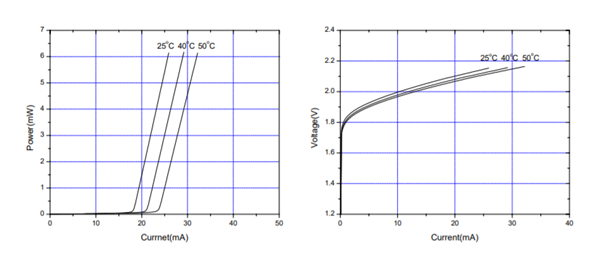
\includegraphics[width=\linewidth]{Fig 1.png}\par
\caption{Graphs taken from the datasheet for the laser diode 2008361. The graph on the left showing the current that can be expected from the photodiode for a given laser with a known power. The graph on the right shows the photo diodes current for a given voltage at a three different temperatures.}
\label{fig}
\end{figure}

\subsection{How to operate lasers when doing experiments}

Because a class 3R laser is being used, safety procedures and practices have been followed, such as: 

\begin{itemize}
    \item When the laser is on, only the operator is in the room.
    \item Laser safety goggles will be worn whenever the laser is on.
    \item If possible, the entire laser beam will be enclosed and separated from the operator of the experiment.
\end{itemize}

\section{Design and implementation}

\subsection{Overview of setup}

When designing, building and testing a laser based FSO. To generate a suitable binary test sequence for the FSLC, a pseudo-random bit sequence (PRBS) will be created using a linear feedback shift register (LFSR) in an FPGA. Once created, it will transmit the PRBS through a laser diode with a maximum output power of 5 mW. Then the signal will be received with a photodiode. The signal will then be amplified and read with the same FPGA. This will be achieved by bouncing the laser beam off a mirror. The BER is then calculated by comparing the received data to the transmitted data and counting the errored bits. The setup for the project can be seen in Fig 2 as well as a top-level diagram showing the how the data moves around the system in Fig 3.
\\\\
The transmitter and receiver use the same clock. Once the system is working, different distances, angles, lasers and transmission speeds can be tested. Then the system can be optimized and tested again to measure the improvements.

\begin{figure}[h]
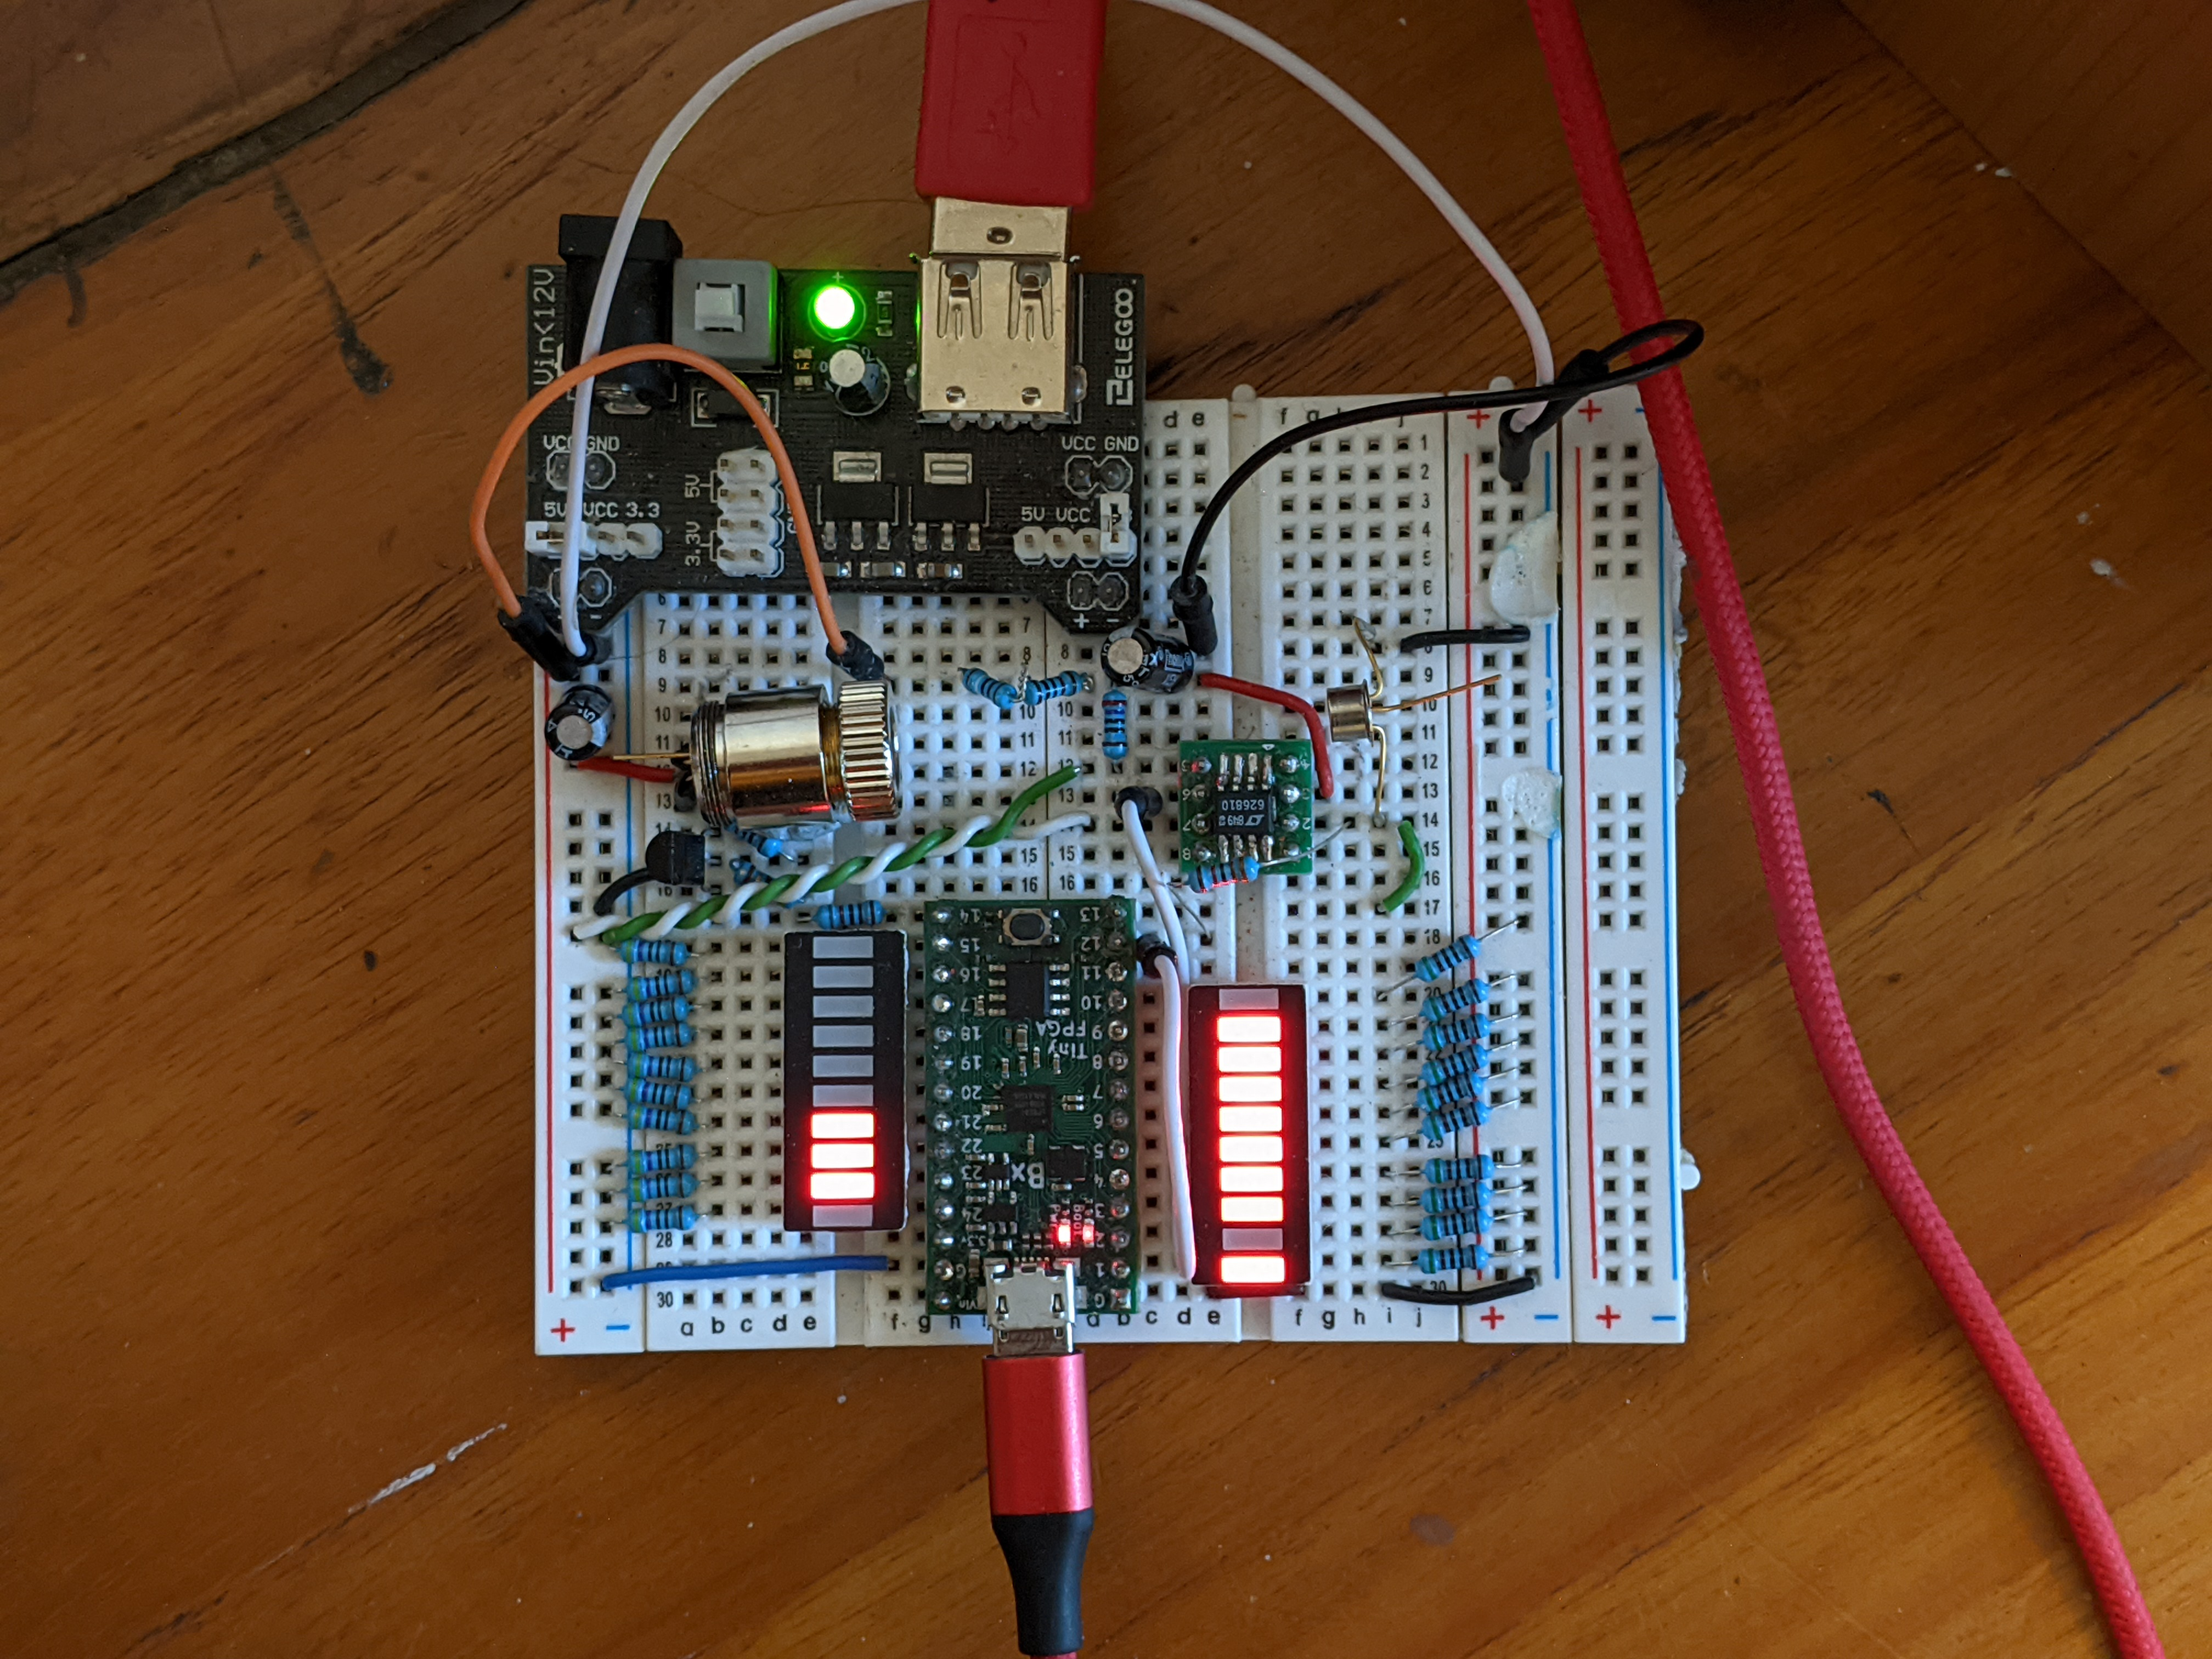
\includegraphics[width=\linewidth]{fig 2.jpg}\par
\caption{Photo of the final setup used in the experiment}
\label{fig}
\end{figure}

\begin{figure}[h]
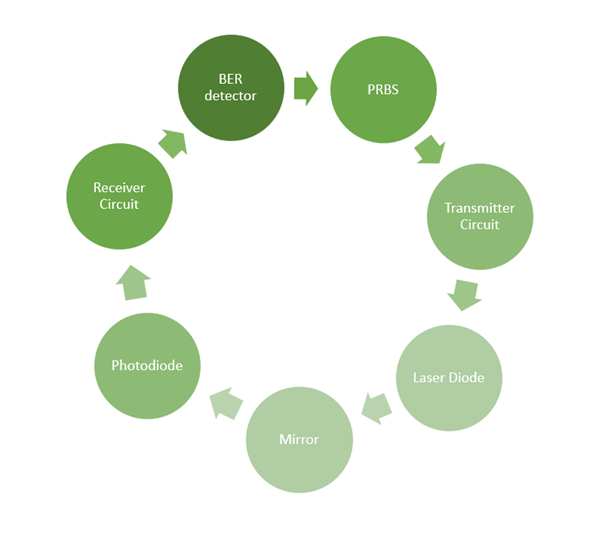
\includegraphics[width=\linewidth]{fig 3.png}\par
\caption{Top level diagram showing the basic elements of the system and the direction and path the data travels in.}
\label{fig}
\end{figure}

\subsection{The transmitter circuit}

For the transmitting circuit, a transistor is used to turn the laser on and off. The transistor selected for this was the KSP10TA (See specifications in Fig 4.) because it has a high gain bandwidth product (650 MHz) and good $h\_{FE}$ (80 when $I\_{c}$ = 25 mA) this means it can operate at the required speed. The laser diode for this circuit is the ADL-65055TL made by Arima Lasers. It was chosen because it is a 5 mW laser, which is the highest output power that is suitable from a safety perspective to be used in the experiment. Its 655 nm typical peak wavelength is useful because it is commonly used, so is easier to find a matching photodiode. It is visible, making it safer to operate, and easier to point the laser beam at the photodiode.

\begin{figure}[h!]
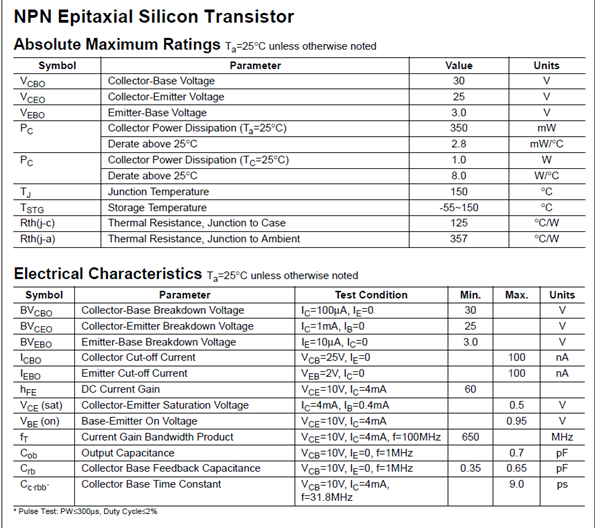
\includegraphics[width=\linewidth]{table 1.png}\par
\caption{Datasheet segment for transistor KSP10TA}
\label{fig}
\end{figure}

The schematic for the transmitter circuit is shown if Fig 5. Note $V\_{in}$ can be either 3.23 V or 0V depending on whether it is at logic level on or off.

\begin{figure}[h!]
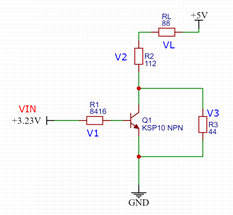
\includegraphics{fig 4a.png}\par
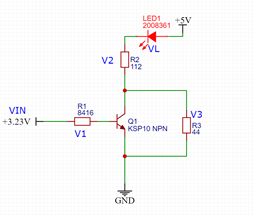
\includegraphics{fig 4b.png}\par
\caption{The transmitter circuit with resistor in place of laser diode (top), with laser diode (bottom)}
\label{fig}
\end{figure}

$R_{1}$ is set to a suitable value to control $I_{b}$ which is the value that, after amplification by the transistor, will be the operational current of the laser diode. If the laser current is 25 mA and $h_{FE}$ is 80, then:

\begin{equation}
I_b\ =\ \frac{I_c}{h_F_E}\ =\frac{25m}{80}\ = 312.5 \mu{}A
%eq1
\end{equation}

\begin{equation}
R_1\ =\ \frac{V_1}{I_b}\ =\frac{V_{in}-\ V_{BE}}{I_b}\ =\ \frac{3.23\ –\
0.6}{312.5\mu{}}\ =\ 8.416 k\Omega{}
%eq2
\end{equation}

$R_{2}$ is used to set the correct operational current and voltage for the laser diode which is 25 mA and 2.2V. Assuming $V_{CB}$ is very small and the transistor is admitting current between collector and emitter. $R_{2}$ can be calculated using kirchhoff's voltage law (KVL) in equation 3:
\\\\
\begin{equation}
R_2=\ \frac{V_2}{I_2}\ =\ \frac{5 - 2.2}{25m}\ =112\Omega{}
%eq3
\end{equation}

By putting the resistor $R_{3}$ between the collector and emitter, there is enough current when the laser is at rest to be just under the threshold current (18 mA). This means the laser can be started faster because the time it takes to get the current up to the threshold is eliminated.

\begin{equation}
R_3=\left(\frac{V_{DD}-V_L}{I_3}\right)-R_2=\left(\frac{5-2.2}{18m}\right)-112=43.5\Omega{}
%eq4
\end{equation}

When building the circuit, to test if the current and voltage is passing through the sensitive laser diode is correct before damaging it. The laser diode is replaced by the resistor $R_{L}$ with the same effective resistance of the laser diode when turned on at 25 mA. The power can be turned on and the current and voltage is tested over the resistor to check the practical values match the theoretical values. This is illustrated in Fig 5. 

\begin{equation}
R_L=\ \frac{V_L}{I_L}=\ \frac{2.2}{25m}=88\Omega{}
%eq5
\end{equation}

The exact component values will be adjusted as needed as calculations are based on typical laser parameters, but they can vary between minimum and maximum values. For example the laser operating current could be as high as 35 mA according to the data sheet.

\subsection{The first receiver circuit}

The schematic in Fig 7 shows the receiver circuit, consisting of the photodetector and a transimpedance amplifier. Note that $C_{1}$ is the parasitic capacitance of the circuit and is very small. The +/- 3.23 V was chosen to power the op amp because there is a stable 3.23 V output from the FPGA board and it is the appropriate voltage according to its data-sheet. 
\\\\
An addition to this circuit may need to be added for it to be able to handle varying power levels as the output level will vary with optical power. If the power level varies significantly during future testing, it will be added. A possible solution to this is a comparator with variable threshold level following the transimpedance amplifier.
\\\\
The photodiode selected for this circuit is the S5972 because it has high photosensitivity at 655 nm wavelength, it also has a high cutoff frequency at 500 MHz, a graph of the photosensitivity over laser beam wavelength can be seen in Fig. 6. The op-amp chosen for this circuit is the LTC6268 because it has a high gain bandwidth product (4 GHz). 

\begin{figure}[h!]
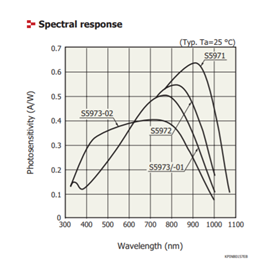
\includegraphics[width=\linewidth]{fig 5.png}\par
\caption{Graph taken from the photodiode S5972 datasheet showing the photosensitivity when lasers with different wavelengths are used with this photodiode.}
\label{fig}
\end{figure}

\begin{figure}[h!]
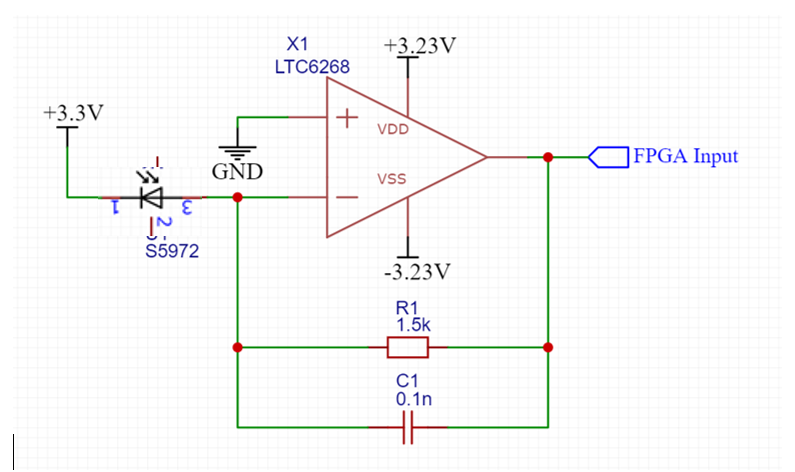
\includegraphics[width=\linewidth]{fig 6.png}\par
\caption{The first Receiver circuit using a transimpedence amplifier}
\label{fig}
\end{figure}

The receiver circuit is designed using a transimpedance amplifier. The photodiode converts the light from the laser beam into current. A transimpedance amplifier converts the current given from the photodiode to the logic high voltage needed to trigger the input of the FPGA. It does this because the inverting and non-inverting inputs of the op-amp effectively want to have the same voltage, but the inverting input wont admit any current because of its very high impedance. So instead, the current is converted into voltage using the feedback resistor $R_{1}$.

Assuming the loss from atmospheric absorption is very low, the current produced when the laser hits the photodiode can be estimated given that the laser is 5 mW and the photosensitivity of the photodiode (A/W) is 0.44 at 660 nm wavelength, then:

\begin{equation}
I_{PD}\ \approx{}\ 5m*0.44=2.2 mA
%eq6
\end{equation}

To calculate the value of $R_{1}$ you divide the high logic level voltage of the FPGA by the current at the photodiode. 

\begin{equation}
R_1=\ \frac{V_{high}}{-I_{PD}}=\ \frac{5}{-2.2m}=2283\Omega{}
%eq7
\end{equation}

After the circuit was built, with many hours spent troubleshooting and debugging, the circuit never gave an acceptable output, so the design was abandoned.

\subsection{Receiver circuit two}

After the first attempt to build a receiver, a simpler design was considered. The design can be seen in Fig 8. This circuit was chosen because of its simplicity and so it could prove that the photodiode, laser and transmitter circuit could all function together and prove that the concept was achievable.\\\\

The circuit works by directly converting the current from the photodiode into voltage using  $R_{L}$. The circuit also includes a low pass filter made from RF and CF to filter out any unwanted high frequency signals in the circuit. 
\\
\begin{figure}[h!]
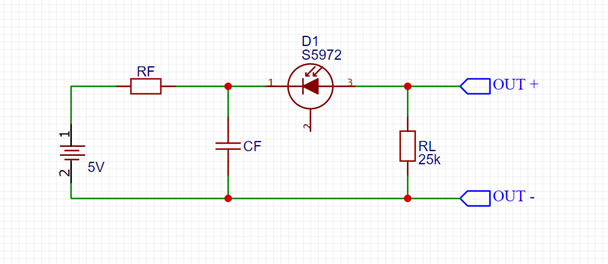
\includegraphics[width=\linewidth]{fig 7.png}\par
\caption{The second receiver design with the real resistor value that was used.}
\label{fig}
\end{figure}

To calculate the theoretical ideal value for the $R_{L}$, equation 8 is used where $V_{o}$ is the logic high of the FPGA. P is the power of the laser beam, in this case 5 mW and R being the responsivity which is the measure of the amps generated by the photodiode for every watt of energy it receives. This number can be found in the data sheet for the Hamamatsu S5971 photodiode and is 0.4 A/W.

\begin{equation}
R_L=\ \frac{V_o}{P*R}=\ \frac{5}{5m*0.4\ }=2.5k\Omega{}
%eq8
\end{equation}

Once the circuit was built the voltage across $R_{L}$ could be measured whilst the laser beam was hitting the photo diode collecting area. The measured voltage was 0.5 V, rearranging equation 8 into equation 9 the real value for the power of the laser beam hitting the photo diode could be calculated. 

\begin{equation}
P=\ \frac{V_o}{R*\ R_L}=\ \frac{0.5}{0.4*2.5k}=0.5mW
%eq9
\end{equation}

Once the real value for the power of the laser beam was calculated, the real value for $R_{L}$ could be calculated using formula 8 giving the value of 25 k\Ω. After rebuilding the circuit with the new value for $R_{L}$ the circuit worked. A set of waveforms were captured using a logic analyzer, as an oscilloscope was not available at the time.
\\\\
Eventually after using a 46 kΩ resistor for $R_{L}$ the circuit managed to operate at a speed of 125 kHz as shown in Fig 10. As the photo diode is a capacitor, the high resistor value causes the time constant to also be high. The high time constant means it takes a long time for the receiver circuit output to go from 0 V to 5 V and from 5 V to 0 V. This can be seen in Fig 10. by the receiver output lagging behind the transmitter waveform. As the project specification it to be able to communicate data at a rate of 1 MHz. Even though the circuit underperformed in terms of speed it did serve its purpose of proving that the concept worked and that a faster receiving circuit needed to be designed.
\\\\
The design in Fig 8 has a RC filter made from $R_{f}$ and $C_{f}$, because the large time constant was the issue and not interference from unwanted frequencies the filter was not used.

\subsection{Third receiver circuit}

The third design is similar to the first receiver circuit, which is a transimpedence amplifier. The main difference between the two being that the photo diode is placed in a photo conductive mode, meaning that it is placed in reverse bias and connected to ground. It essentially creates negative current. The non-inverting input is set to a low voltage by the voltage divider made from $R_{6}$ and $R_{7}$ in Fig 9, this stops the output from being saturated.

\begin{figure}[h!]
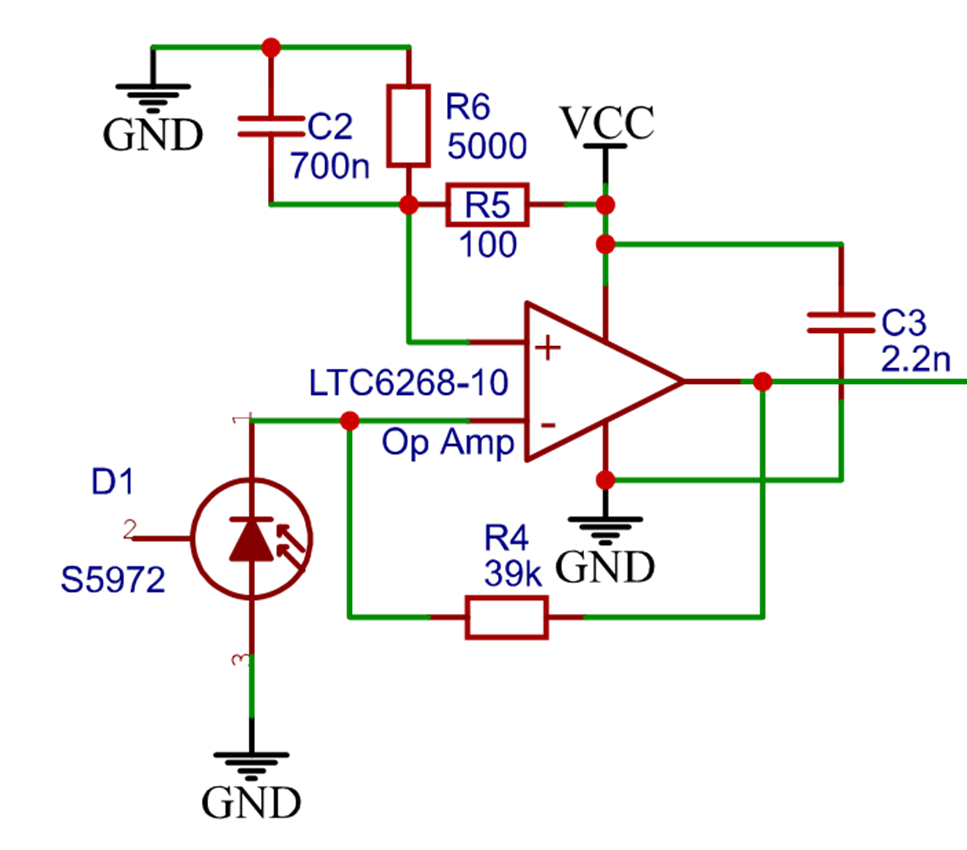
\includegraphics[width=0.8\linewidth]{fig 10.png}\par
\caption{The transimpedance amplifier in photoconductive mode and the third receiver circuit built for the project.}
\label{fig}
\end{figure}

To calculate $R_{4}$ we use equation 10 $V_{out(max)}$ is the logic HIGH voltage specified by the FPGA and $V_{out(min)}$ is the logic LOW specified by the FPGA. $I_{pd}$ is the current created by the photo diode with the laser beam hitting it. $I_{pd}$ was measured creating a physical value to work with. After the circuit was built the logic HIGH output was not high enough to be comfortably above the threshold of the FPGA, so a 39k resistor was used.

\begin{equation}
R_4=\frac{V_{out(max)}-\ V_{out(min)}}{I_{pd}}=\
\frac{5-0.1}{150\mu{}}=32.6k\Omega{}
%eq10
\end{equation}

Usually, transimpedance amplifiers in photo conductive mode use small capacitors in parallel with $R_{4}$ in order to stabilize the signal by compensating for the capacitance of the photo diode. A capacitor was not placed in parallel with $R_{4}$ in this circuit however because it seemed the capacitance's present in the breadboard and components where sufficient and offered the best performance. At first, the ideal capacitance was calculated using formula 11 where $f_{p}$ is the frequency that data is being transmitted, giving the value of 4 pF. 
\\\\
After testing and incrementally reducing the size of the capacitor, the parasitic capacitance was found to be enough to stabilize the signal and give the best performance because it reduced the time constant, which in turn increases the bandwidth. The circuit could be improved further by moving the circuit onto a perfboard or a custom PCB reducing the parasitic capacitance further, although improved performance on that front is not guaranteed because the signal might become too unstable. 

\begin{equation}
C_{feedback}=\ \frac{1}{2*\pi{}*R_4*f_p}=\frac{1}{2*\pi{}*32.6k*1M}=4.88pF
%eq11
\end{equation}

$C_{2}$ from the circuit in Fig 9 was calculated using formula 12 where $f_{c}$ is the corner frequency and in this case was chosen to be 580 Hz. 

\begin{equation}
f_c=\frac{1}{2*\pi{}*C_2*(R_5\vert{}\vert{}R_6)}=\frac{1}{2*\pi{}*700n*390}=580Hz
%eq12
\end{equation}

A decoupling capacitor $C_{3}$ was placed between the positive and ground power supply to the op-amp acting as a decoupling capacitor. Usually, two decoupling capacitors are used with values of 10 µF and 0.1 µF. After testing, one 2.2 nF capacitor was found to be the most effective Fig 12(top) shows the output signal of the op amp without the 2.2 nF capacitor and Fig 12(bottom) shows the output signal with the 2.2 nF capacitor.

\begin{figure}
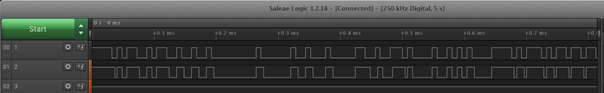
\includegraphics[width=\linewidth]{Fig 9.png}\par
\caption{The second receiver circuit operating at a 125kHz bit rate at a distance of 2.7cm. The waveform at the top is the signal coming from the FPGA and the bottom waveform is the signal coming from the receiver output.}
\label{fig}
\end{figure}

\begin{figure}
\includegraphics[width=\linewidth]{Fig 13.png}\par
\caption{Output from Quartus II simulation of 4-bit LFSR}
\label{fig}
\end{figure}

\begin{figure}[h!]
\centerline{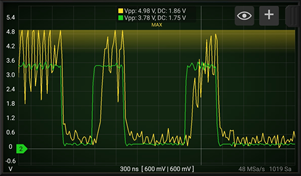
\includegraphics[width=0.8\linewidth]{fig 11a.png}}\par
\centerline{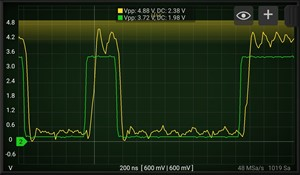
\includegraphics[width=0.8\linewidth]{fig 11b.jpg}}\par
\caption{(top) without capacitor and (bottom) with capacitor. In both figures the yellow waveform is the output signal from the third receiver circuit and the green waveform is the output signal from the FPGA that is the input signal into the transmitter circuit.}
\label{fig}
\end{figure}

\subsection{Pseudo random bit sequence generation}

A PRBS is a binary sequence built in blocks of bits. For example a 4-bit RPBS would be in blocks of 4 bits. The PRBS will display every combination the 4 bits could represent apart from 0000. The PRBS does this without ever repeating the same 4-bit value. This is useful in testing the validity of a communications system because you can ensure that every combination of bits will be tested.
\\\\
When Designing the PRBS generator, firstly a 4-bit LFSR was built in Quartus II as seen in Fig 13. 
Then the circuit was simulated to check that it was functioning correctly, as shown in Fig 11. \\

\begin{figure}[h!]
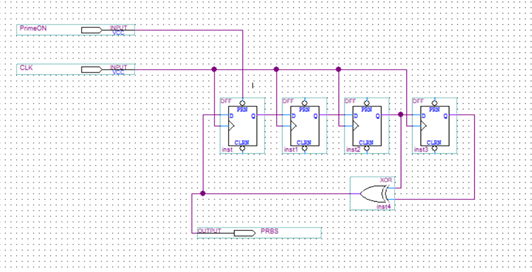
\includegraphics[width=\linewidth]{fig 12.png}\par
\caption{4-bit LFSR circuit in Quartus II}
\label{fig}
\end{figure}


After the 4-bit PRBS was found to function properly an 8-bit LFSR and a 32-bit LFSR was built in Verilog (see Appendix 11.1. and 11.2.) so it could be used in the FPGA. Once programmed, a simple circuit was built (seen in Fig 14.) to test if it worked, a logic analyzer was used to record the output of the LFSR and is shown for the 8-bit and 16-bit LFSR [10]
\\
\begin{figure}[h!]
\centerline{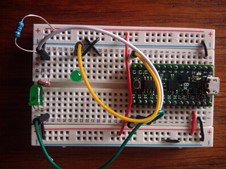
\includegraphics[width=0.9\linewidth]{fig 14.jpg}}\par
\caption{Simple circuit built to test Verilog code}
\label{fig}
\end{figure}

Eventually, a 10-bit PRBS was selected because it could complete a cycle in one tenth of a second, which was useful when testing because it could be relied upon that the laser had not moved out of position in that time frame. 
\\\\
To fully confirm that the circuit was outputting the correct binary sequence, a spreadsheet was generated as shown in Fig 16. Using logic operators, where cell 3A uses the command “=--xor(G2,J2)” which represents an XOR gate in between cells G2 and J2. This command was applied to all the subsequent A cells beneath. Every other cell after cell 3A copies the value of the cell above and to the left of itself (e.g. cell B3 is “=A2”). Using the self-filling feature in Google Sheets by highlighting the entire row and dragging the tab in the bottom right of the cell in the downward direction all 1023 lines can be filled very quickly. 
\\\\
To verify that this table, and in turn the 10-bit LFSR, was accurate, another table was created. This table added all the zeros and ones as shown in Fig 15. This table shows that there are almost an equal number of ones and zeros, with there being an extra one for each cell of the shift register. The reason there is one less zero for every register in the shift register is because this LFSR omits the value 0000000000. Fig 15 when compared to the testbench shown in fig 11 shows that the LFSR and the Verilog code are working optimally. 

\begin{figure}[h]
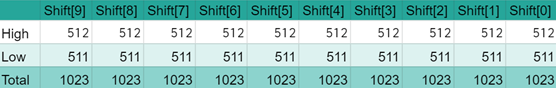
\includegraphics[width=\linewidth]{table 2.png}\par
\caption{This table shows that the LOWs in each column in the table in Fig 17. are equal to the total number of HIGHs minus one.}
\label{fig}
\end{figure}

\begin{figure}[h]
\centerline{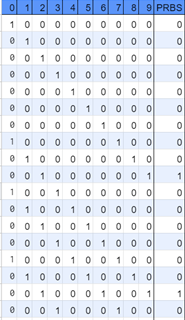
\includegraphics[width=0.4\linewidth]{table 3.png}\par}
\caption{Truth table for the first 18 values from the 10-bit LFSR}
\label{fig}
\end{figure}


\begin{figure}
\includegraphics[width=\linewidth]{Fig 19.png}\par
\caption{This testbench output shows that the output from the 10-bit LFSR circuit is the same as the table in Fig 16.}
\label{fig}
\end{figure}

\subsection{BER detector}

To know how effective the circuit is, the BER needs to be calculated. The BER is a numerical ratio of errors that occur in a communication system. For example, a BER of 0.001 means there is one error for every 1000 bits sent.
The BER is calculated by counting the total number of errors. The total number of errors means the total number of times the signal picked up by the receiver is different from the signal sent from the transmitter circuit. For example, a HIGH state signal is sent, and a LOW state is received. 
\\\\
The detection of these errors is done in the FPGA and the code that completes the task is shown in Fig 18. In the section labeled “Competitor”, on line 121, i\_ReceivedSignal is the signal from the receiver and o\_PRBS is the signal sent from the transmitter. \\

The operator \^{} represents an XOR gate meaning if they are both High or both LOW then the variable w\_Error will be HIGH otherwise when both signals do not match it is set too LOW. Note the matches are also counted on line 120 to the variable w\_Match. The \~{} symbol representing a NOT gate, so giving the opposite value to w\_Error.\\\\

To obtain the total number of errors, the FPGA needs to be told when to stop counting them. \\\\

This is done with the always block starting on line 93 in Fig 18. Line 104 takes the sum of the errors and matches which are equal to the total number of bits sent. \\\\

Every possible combination of bits has been sent when the number of bits sent is 1023. \\\\

Line 109 checks if 1023 bits have been sent and that it is the first time they have been sent.\\\\

Once 1023 bits have been send then the number in the r\_AddErrorCounter register is stored in the r\_TotalErrors register. r\_TotalErrors is a 10-bit number and the bits are displayed using 10 LEDs. After the number is displayed it is recorded in Excel in a document that automatically calculates the BER using the total errors over the number of bits sent, so 1023 for each test. The reason the last bit of calculation was done in Excel is because using and representing fractions inside the FPGA was overly complicated for the application and the data would have been added to Excel regardless. 

\begin{figure}[h]
\centerline{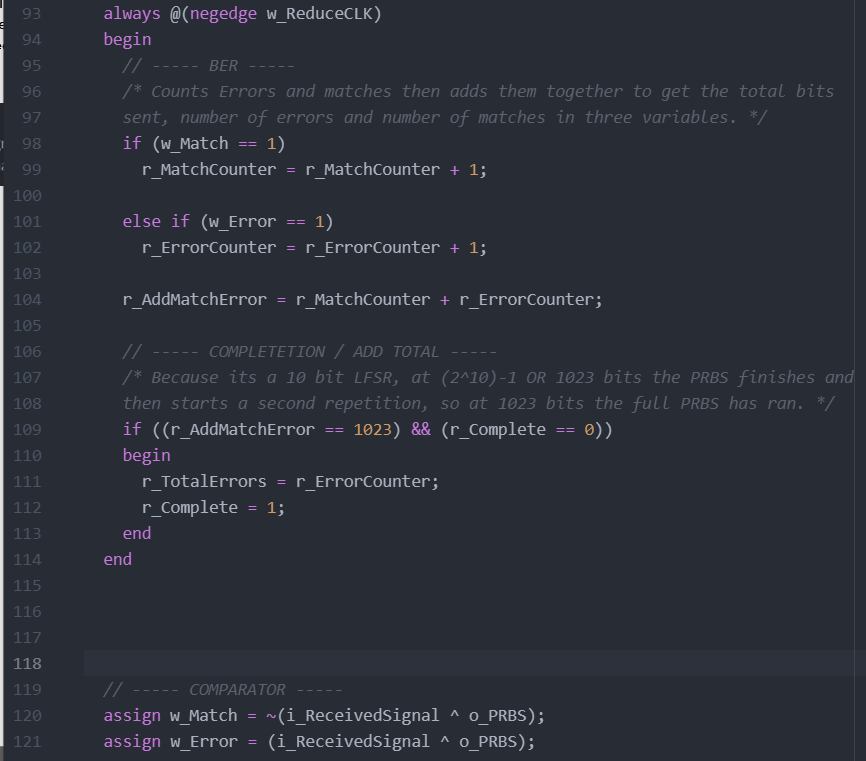
\includegraphics[width=\linewidth]{fig 20new.png}\par}
\caption{Section of the Verilog code used in the FPGA to detect transmission errors}
\label{fig}
\end{figure}

An early version of the BER generator used a comparator, which worked just like the r\_AddMatchCounter mentioned above, so that if tx and rx are the same when r\_Comp is high. Fig 19 shows a test done to check the comparator is working. The top signal is the reduced clock at a frequency of 2 kHz. Below that is the transmitted signal followed by the received signal, and at the bottom the signal from the comparator. \\\\

In the sections before and after the section indicated by the red arrows, the comparator is always HIGH at the negative edge of the clock. The section in between the red arrows is where a finger was placed in between the laser and the photodetector interrupting the flow of data. Notice in this section that whenever the transmitter signal is HIGH an error should occur because the received signal is permanently LOW. \\\\

The comparator is known to be working because it does in fact show an error at the negative edge of the clock at every point the transmitter is HIGH. When this test was carried out the number given by the r\_TottalErrors register was 44, after counting the same number errors manually in the wave diagrams, it was known that the comparator was functioning properly.

\begin{figure}[h]
\centerline{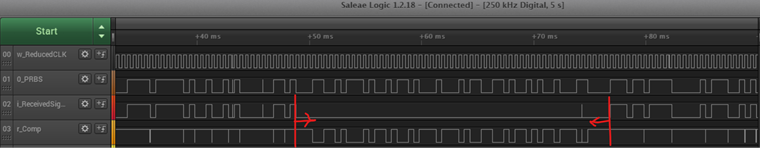
\includegraphics[width=\linewidth]{fig 21.png}\par}
\caption{Shows the test done to check the comparator is operating correctly.}
\label{fig}
\end{figure}

\subsection{Lens selection}

The light, when it leaves a laser diode it is not perfectly strait. It diverges at a known rate called a divergence angle. This means that a photodiode detecting this light from a distance will only receive a fraction of the power transmitted. This makes the data hard to read, because the signal will be subject to greater amplification, which in turn will sacrifice the maximum speed at which the data can be transmitted.\\\\ 
If there is a need to amplify too much, there is a risk that the data will be unrecoverable because it cannot compete with the background noise. To solve this issue, a culminating lens placed in front of the laser beam at a distance known as the focal length, as shown in Fig 20. This reduces the divergence angle greatly.  A culminating lens can also be placed in front of the photodiode, focusing the diverged beam into the photosensitive area of the photodiode.

\begin{figure}[h]
\centerline{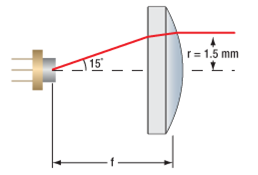
\includegraphics[width=\linewidth]{fig 22.png}\par}
\caption{The set up for a culminating lens when used with a laser diode}
\label{fig}
\end{figure}

To calculate the focal length, both the divergence angle of the laser and the radius of the photosensitive area needs to be found from the data-sheets of the laser diode and photodiode. Then the following equation is used to find the correct focal length:

\begin{equation}
f=\ \frac{r(m)}{tan⁡(\frac{\theta{}}{2})}=\
\frac{0.4mm}{tan⁡(14^\circ{})}=1.6mm
%eq13
\end{equation}

Next, we need to calculate the numerical aperture of the laser diode by using the following equation:

\begin{equation}
{NA}_{diode}\approx{}\sin{\left(14^\circ{}\right)}=0.24
%eq14
\end{equation}

If we are just using the full width at half maximum (FWHM) to illustrate the beam diameter then having $NA_{lens}$ $>$ $NA_{diode}$ is enough. If, however Gaussians beam profile is used instead of the FWHM, using a $1⁄e^{2}$   beam diameter. Then using a $NA_{lens}$ 	$\approx$ 2*$NA_{diode}$ will capture more of the transmitted power than would have been lost due to far field diffraction [11]. \\

After all these calculations and selecting a suitable lens, it was clear that acquiring a specific lens was too expensive for this project. So instead, a culminating lens was taken from a cheap laser pointer of a similar wavelength and used. This lens was reasonably effective and was a lot better than no lens at all, but it was less effective on the laser diode chosen for the project than the laser it came from. \\

One culminating lens was placed close to the laser diode in the tests. If a second set of tests were to have been done, a second lens would have been place in front of the photodiode.

\section{Results and discussion}

Once the circuit was functioning, several tests were carried out to assess the performance of the system. The exact configuration of the circuit is shown in Fig 21. The third receiver circuit is used, LED2 to LED11 show the total number of errors and LED12 to LED21 are used for debugging.

\begin{figure}[h]
\centerline{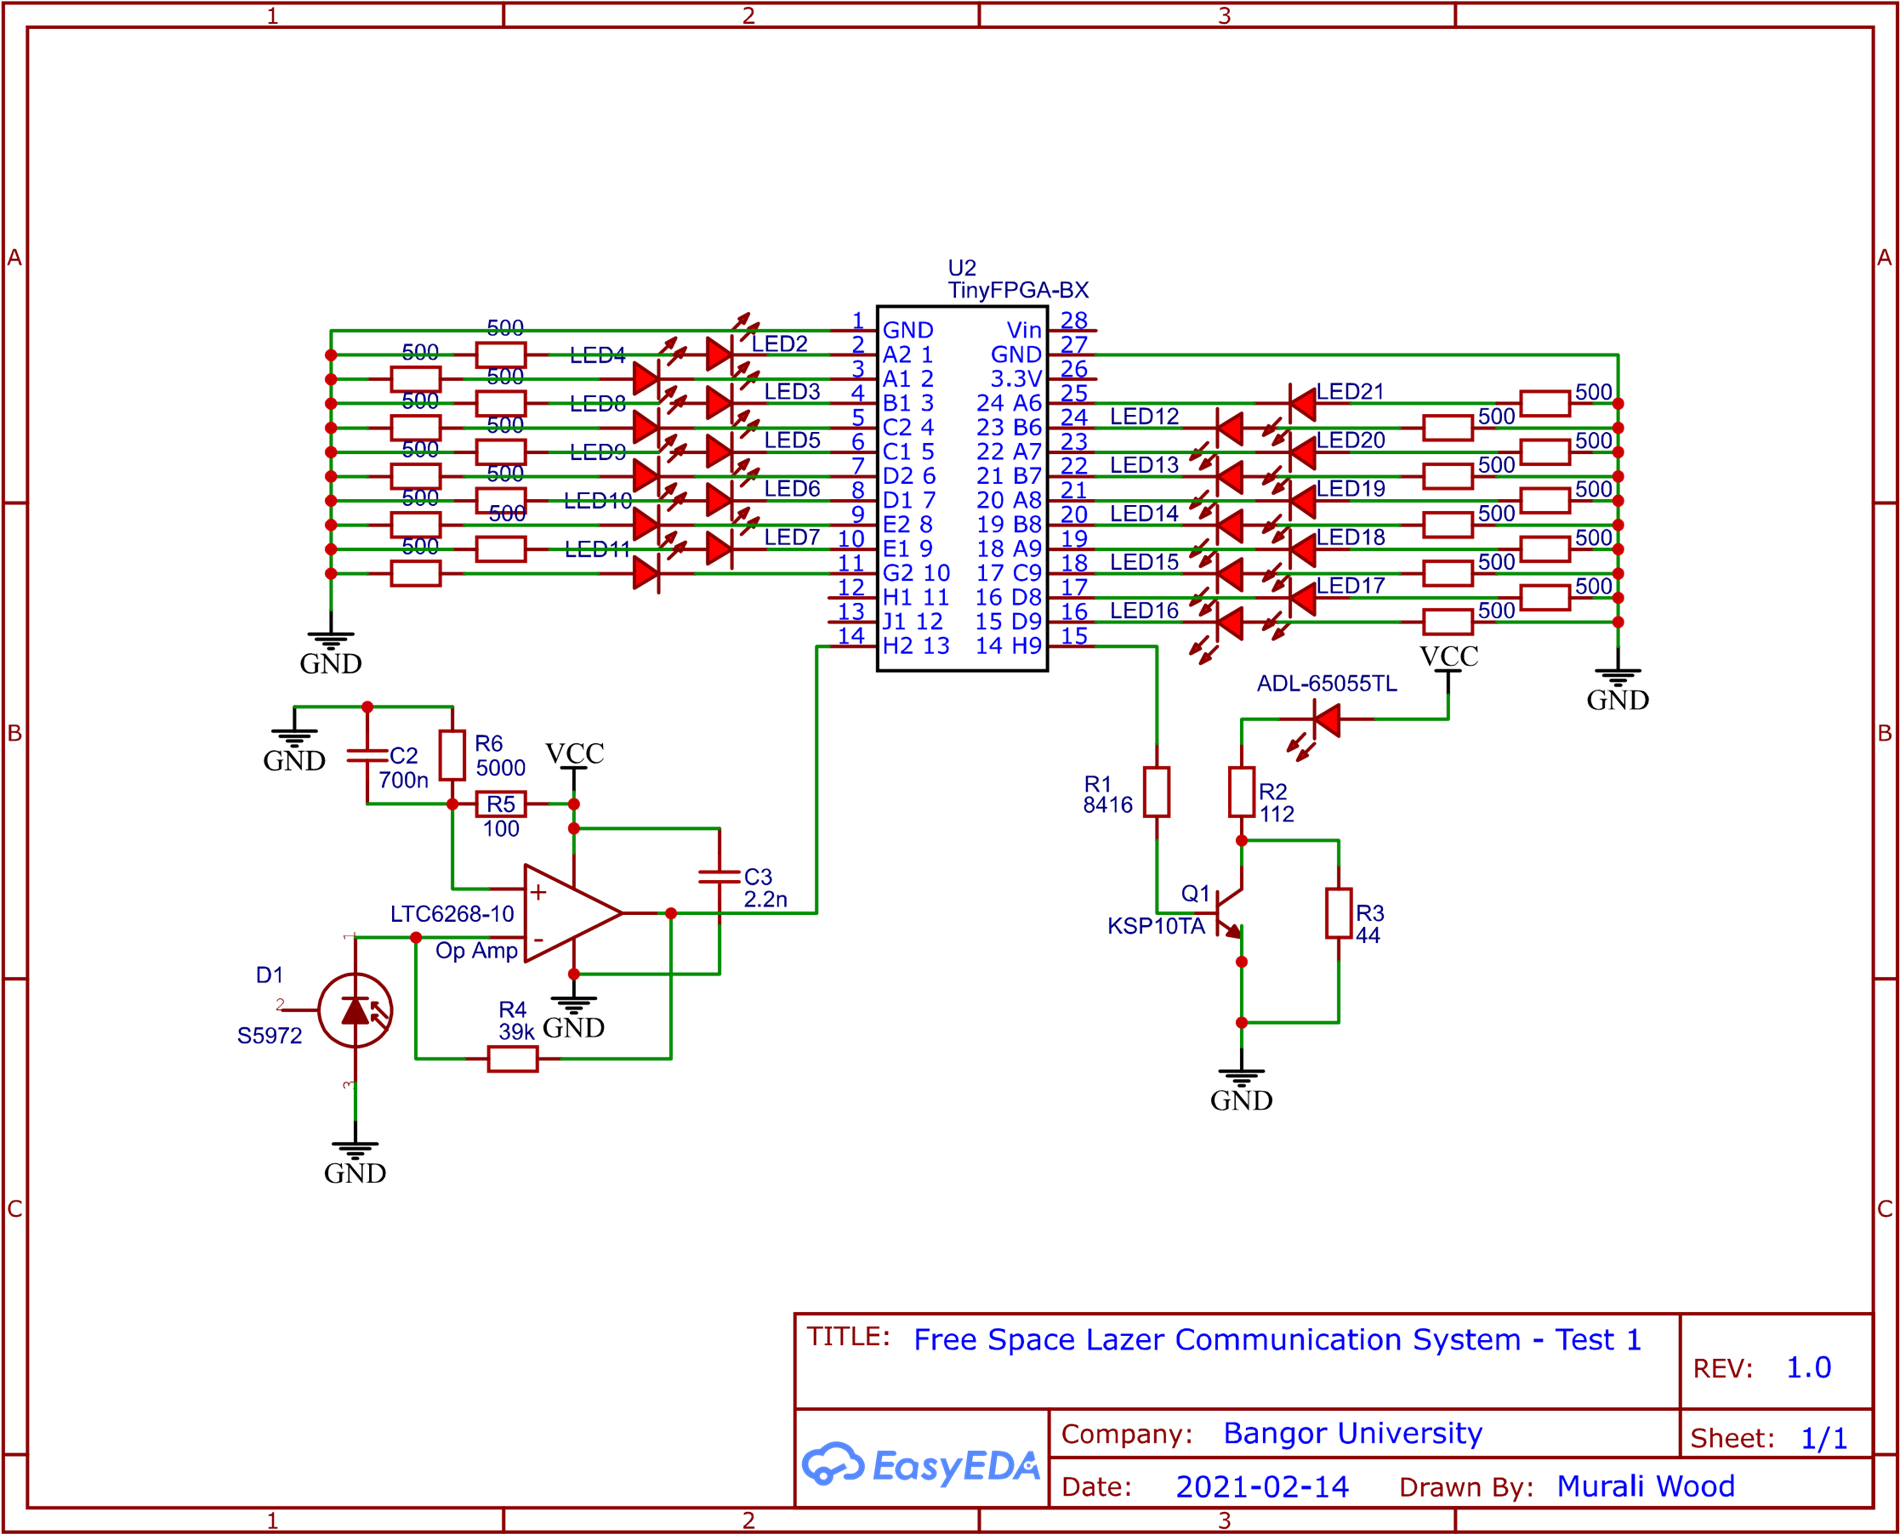
\includegraphics[width=\linewidth]{fig 23.png}\par}
\caption{This is the complete and final circuit, which was used when testing.}
\label{fig}
\end{figure}

\subsection{BER variation with bit rate}

The first set of data collected was the performance at different transmission rates. The receiver was placed 3 cm away from the transmitter at 0 degrees off axis. Starting at 700 kbps 10230 bits where sent in 10 sets of 1023 bits then the BER is automatically calculated in the document. The results can be seen in fig 22 and are graphed in Fig 23. 
\\\\
The results show that the system operated with a BER under 0.001 at bit rate of up to 2.6 Mbps, having a BER under 0.001 is considered acceptable in many use cases. Above 2.6 Mbps the BER is in between 0.19 and 0.24 which suggest that the system is still correct sometimes because if it were purely left to chance, a BER of 0.5 would be expected. This test revealed where the limits are for the system. If further tests where to be done they should be done between 2.6 Mbps and 2.7 Mbps to locate to a more precise degree of where the limit is.

\begin{figure}[h]
\centerline{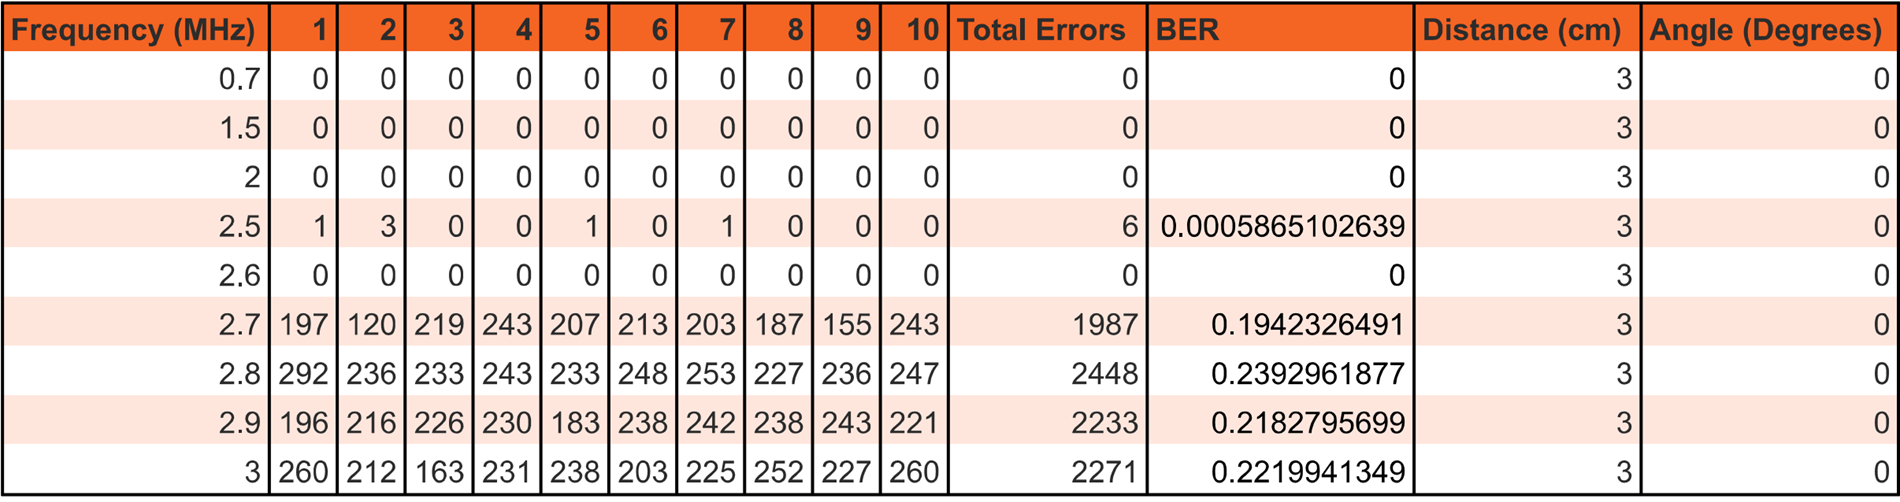
\includegraphics[width=\linewidth]{table 4.png}\par}
\caption{shows the BER over bandwidth at a distance of 3cm}
\label{fig}
\end{figure}

\begin{figure}[h]
\centerline{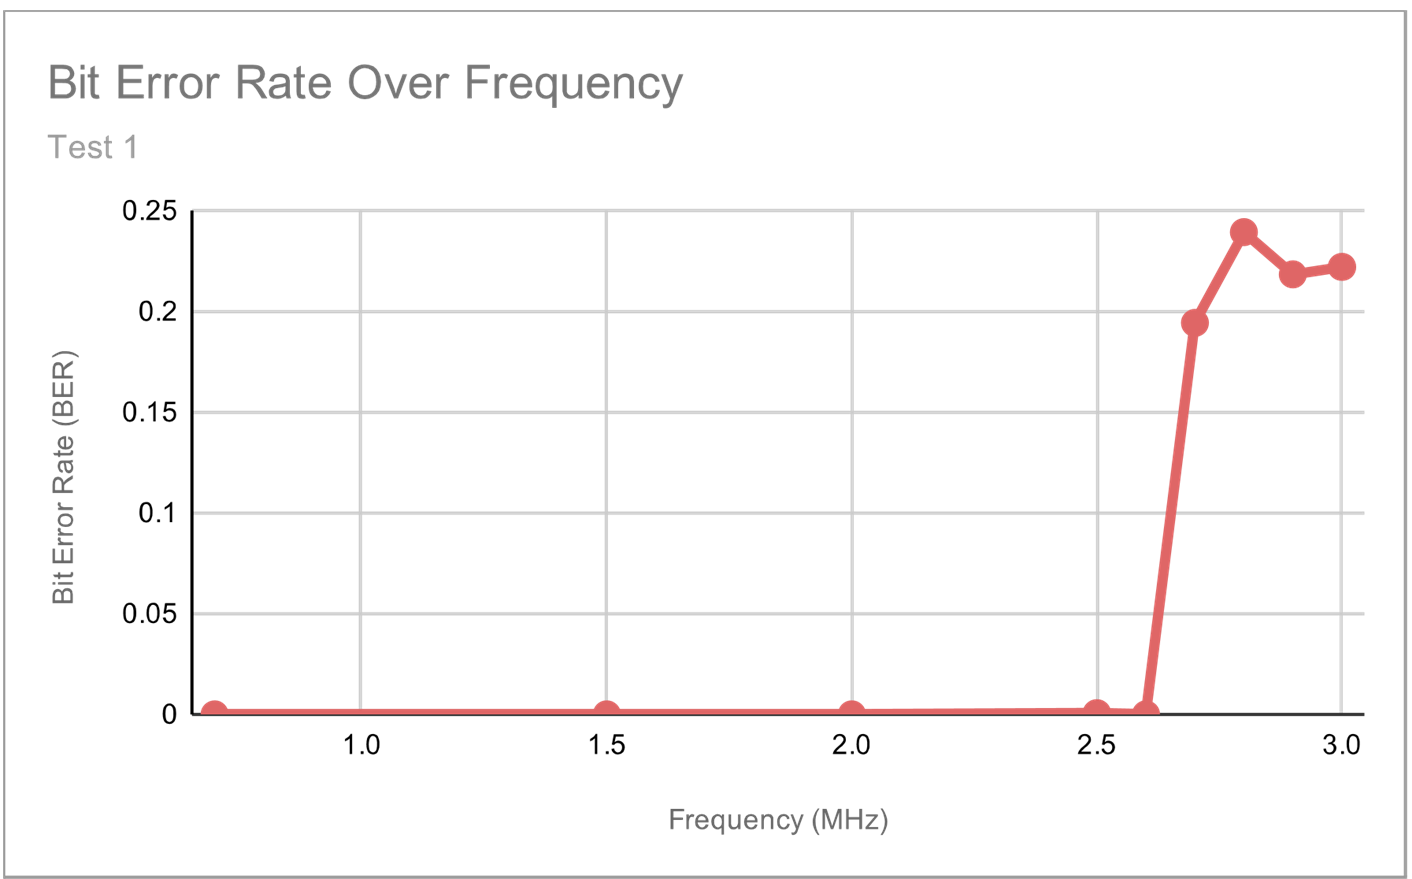
\includegraphics[width=\linewidth]{fig 24.png}\par}
\caption{Shows a graph of the BER over bit rate at a distance of 3cm}
\label{fig}
\end{figure}

\begin{figure}[h]
\centerline{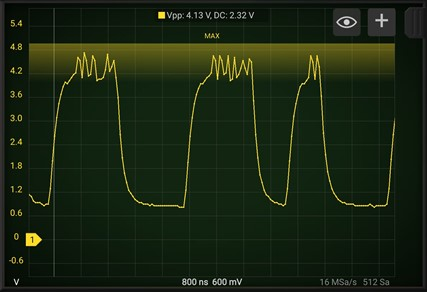
\includegraphics[width=\linewidth]{fig 25.jpg}\par}
\caption{Waveform of test at 1.5Mbps}
\label{fig}
\end{figure}

\subsection{BER over angle}
The angle of the laser beam, with respect to the photodiode, was incrementally changed and the performance was measured. After determining that the maximum bit rate the system was capable of was 2.6 Mbps a transmission speed of 2 Mbps was selected. 2 Mbps was selected because it was assumed to show the variation in performance at different angles. The test was carried out at a distance of 3 cm where the photodiode started off in line, or pointing directly at the laser. This starting position was set as 0 degrees and the other measurements were taken as the difference in angle between it and the original position.\\\\

In fig 25 and Fig 26 we can see the results. There are no errors at all from 0 to 53 degrees. The reason for his is that the transmission speed of 2 Mbps was too low to see a change in errors as the angle increases. A transmission speed of 2.6 Mbps should have been selected. At 63.4 degrees, the only angle to register errors, half the laser beam was obstructed by the outer case of the photodiode, reducing the power collected by the photodiode and reducing the output voltage of the op-amp to below the threshold voltage of the FPGA, therefore causing a high number of errors

\begin{figure}[h]
\centerline{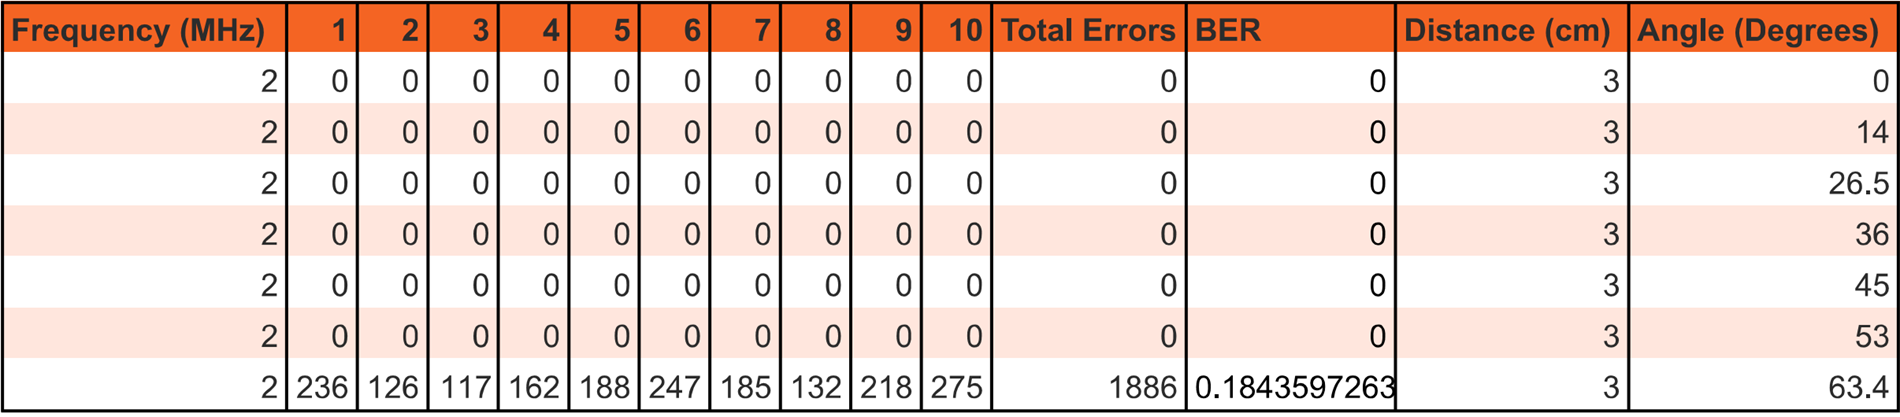
\includegraphics[width=\linewidth]{table 5.png}\par}
\caption{shows the BER over angle at a distance of 3cm}
\label{fig}
\end{figure}

\begin{figure}[h]
\centerline{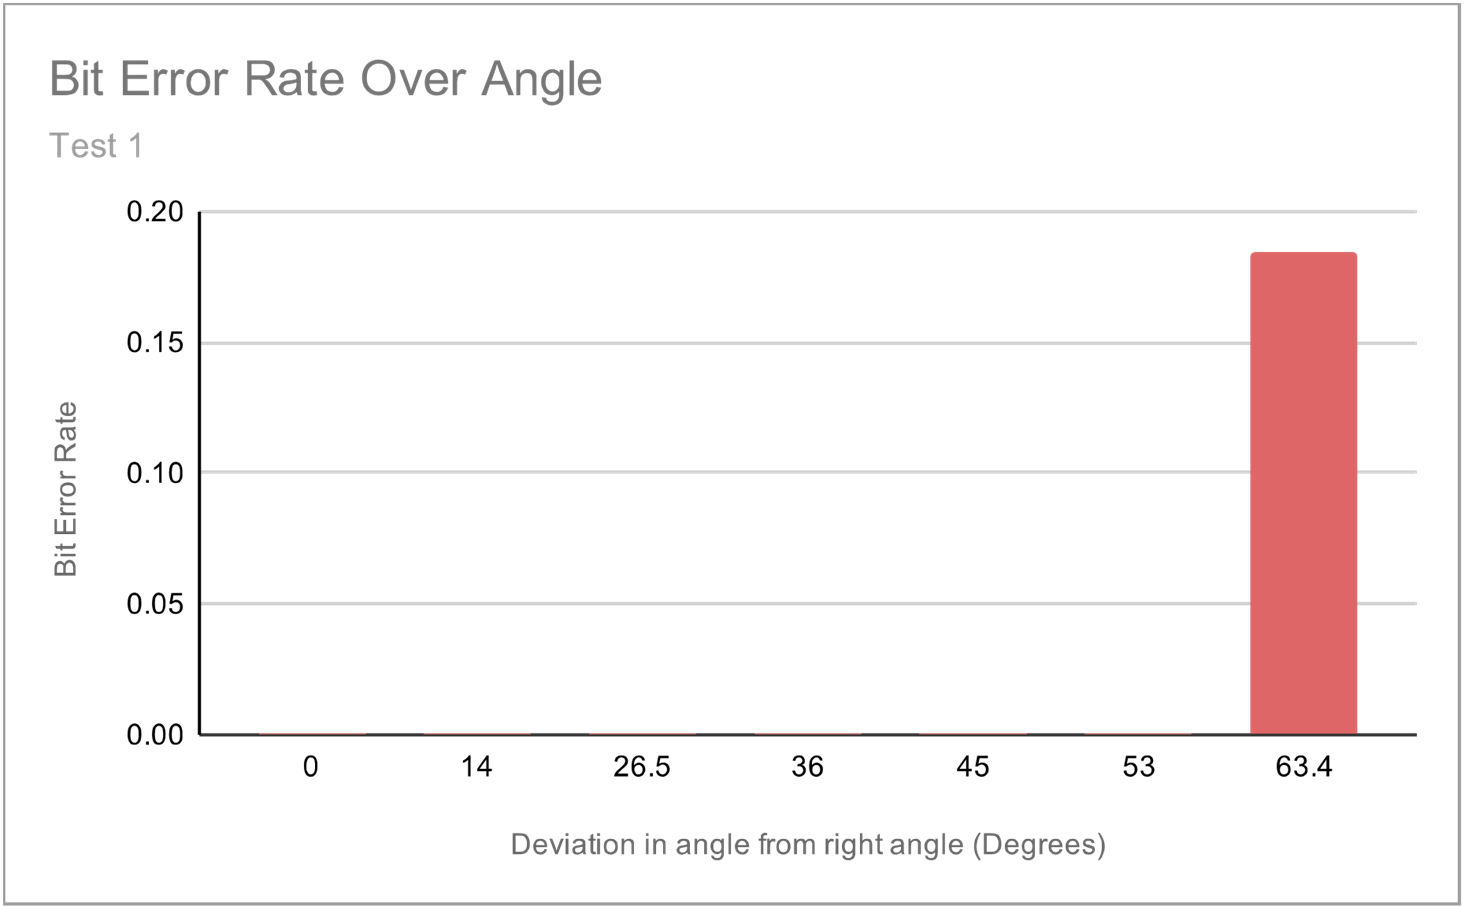
\includegraphics[width=\linewidth]{fig 26.png}\par}
\caption{Shows a graph of the BER over angle at a distance of 3cm}
\label{fig}
\end{figure}

\subsection{BER over distance}

For the test of BER over distance, the transmission speed of 2 Mbps was selected to keep the experiment to a manageable distance, and an off-axis angle of 0 degrees was selected to keep things consistent. The results are shown in Fig 27 and graphed in Fig 28. 
\\\\
The results show that the system works with an acceptable BER for distances up to 65 cm. The reason errors happen more frequently after 65 cm is that the beam diverges to a point where its area is bigger than the photo sensitive plate on the photodiode and, therefor, not all the energy is collected causing the signal to flatten to a point that it is below the threshold voltage. 
\\\\
The results from the test at 23 cm show an anomaly where test 3 shows 23 errors which varies greatly from the average of 0.56 errors for the other 9 values. The anomaly is due to the laser beam not being centered on the photodiode properly, thus dropping the voltage of the logical HIGH closer to the voltage threshold causing false LOW values. A similar thing happened on the 69 cm test for test 4.
 \\\\
If further tests could have been carried out, it would have been interesting to see how far the circuit performed at a 1 Mbps transfer rate as that was the target specification. I would also be interested to see in more detail, what happens at the at the point where errors start to occur at around 65cm, if data could be collected with a smaller sample period in that region, we might see a smoother exponential type transition. 
\\\\
To increase the distance further, a second culminating lens was planned to be placed in front of the photodiode, facing in the opposite direction to the culminating lens on the laser diode. This would collect the laser beam that has diverged to a point where it is larger than the photosensitive plate of the photodiode, and reduce its area, allowing the photodiode to collect all the power of the laser beam minus the efficiency losses from the lens.

\begin{figure}[h]
\centerline{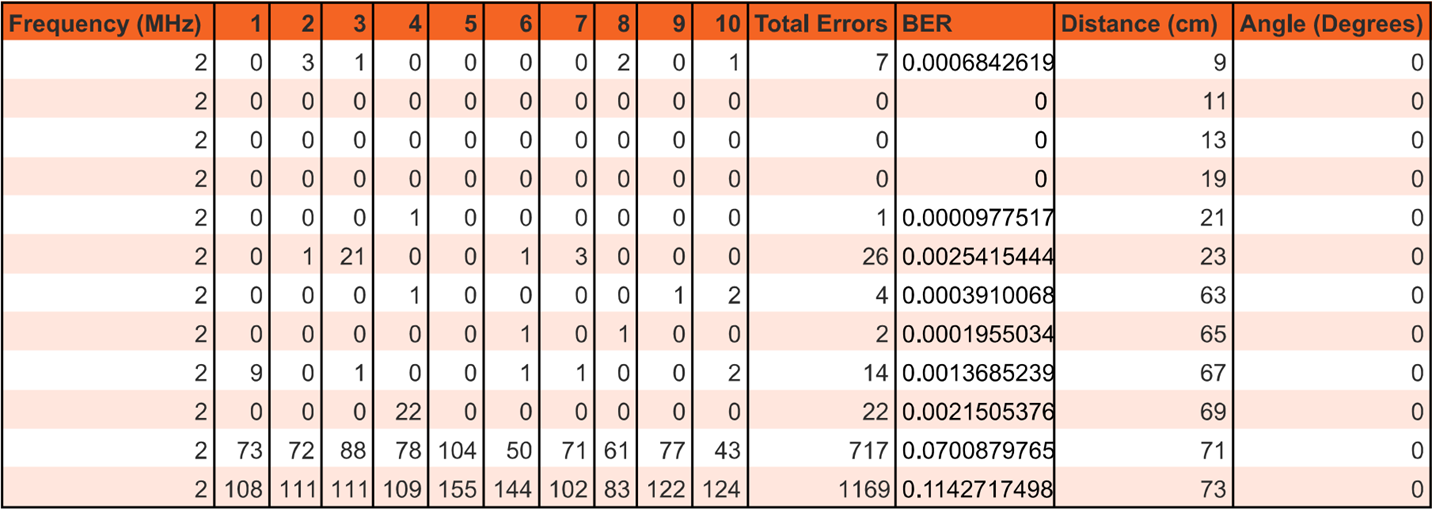
\includegraphics[width=\linewidth]{table 6.png}\par}
\caption{shows the BER over distance at a bit rate of 2Mbps}
\label{fig}
\end{figure}

\begin{figure}[h]
\centerline{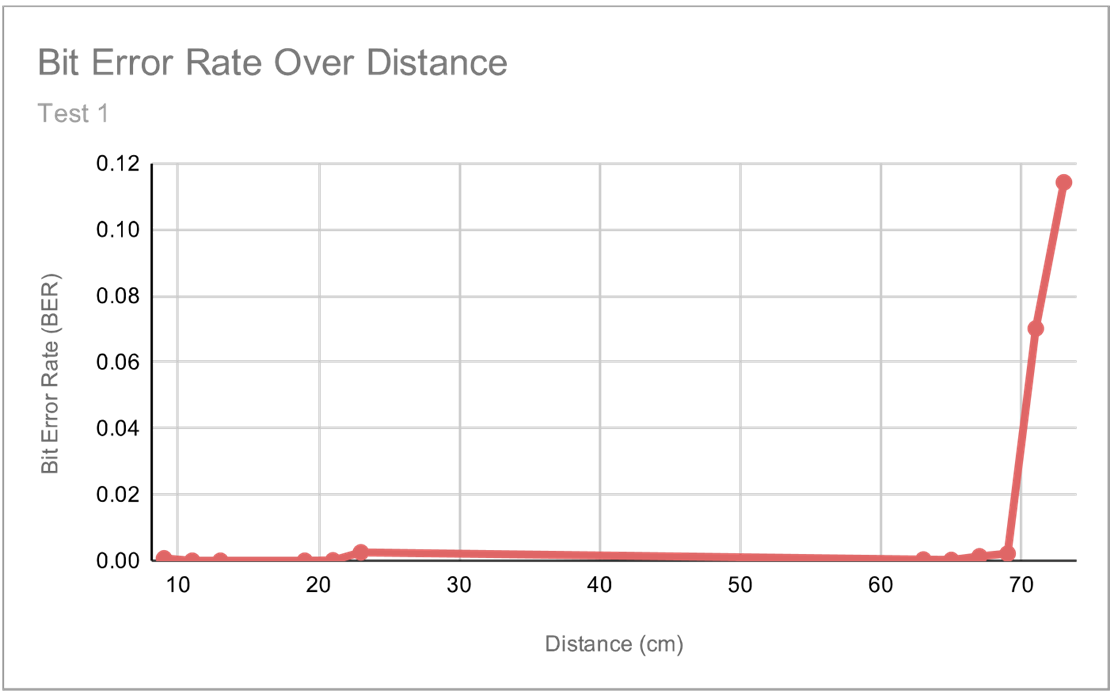
\includegraphics[width=\linewidth]{fig 27.png}\par}
\caption{Shows a graph of the BER over distance at a bit rate of 2Mbps}
\label{fig}
\end{figure}

\section{Conclusion}

Through finding and ordering the components, designing the transmitter and receiver circuits, calculating the culminating lens, extensively reading the data-sheets for the components, programming LFSR and BER, building the circuit and testing it the following conclusions can be drawn from this project:

\begin{itemize}


    \item 	This project has proved that making a LFSC device out of, off the shelf parts and using nothing more than a cheap oscilloscope that runs on an android app and no bench top power supply, is possible. A device that can communicate at 2 Mbps at distances of 65cm and at bit rates of up to 2.6 Mbps.

    \item   It seems with only one culminating lens, one meter is difficult, but may be possible with an expensive lens, and if 2 culminating lenses are used then even greater distances could be achieved.

    \item	The angle of the beam hitting the photodiode does not have a great effect on the device’s performance, but further tests should be done to determine the extent in greater detail.
\end{itemize}

\section{Future work}

Due to the pandemic, the use of an oscilloscope that generates an eye diagram was not available. If one had been available, we could have used it to determine the best place to set the threshold voltage, by finding the widest part of the eye diagram labeled in green in Fig 29. To do this a voltage comparator can be implemented along with a high-speed op-amp to amplify the signal to the logic HIGH voltage of the FPGA. The LTC6268-10 like the one used in the receiver circuit would be a good candidate for this. \\\\

The eye diagram can also be used to determine the best time to sample its state, looking at the orange arrow in fig 29. where the tallest section of space inside the eye of the diagram is. This indicates the point in time to sample from to achieve the least number of errors. \\\\

To sample from this point, a second clock needs to be created inside the FPGA that is several times faster than the bit rate. Then a counter counts the new clock's signal, restarting every time the bit rate clock changes state. They, by referring to the eye diagram match the number of the counter to the point in time where the orange marker is, And use that number on the counter as the trigger for when to record the received signal. \\\\

Once these changes have been implemented, further tests to measure their improvements would be worthwhile.

\begin{figure}[h]
\centerline{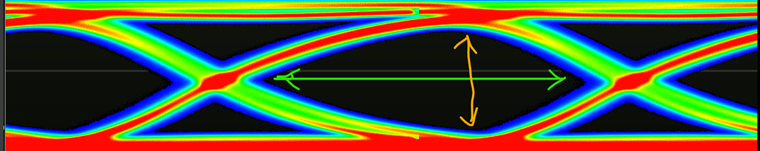
\includegraphics[width=\linewidth]{fig 28.png}\par}
\caption{An example of an eye diagram for illustrative purposes. (This is not a signal taken from this project.)}
\label{fig}
\end{figure}

Further investigation into using a second culminating lens would be beneficial. By placing a culminating lens in front of the photodiode, the laser beam can be focused onto the photosensitive area of the photodiode, preventing the loss of power from diffracted light failing to be collected. A photo of the setup for the preliminary tests for this can be seen in fig 30.

\begin{figure}[h]
\centerline{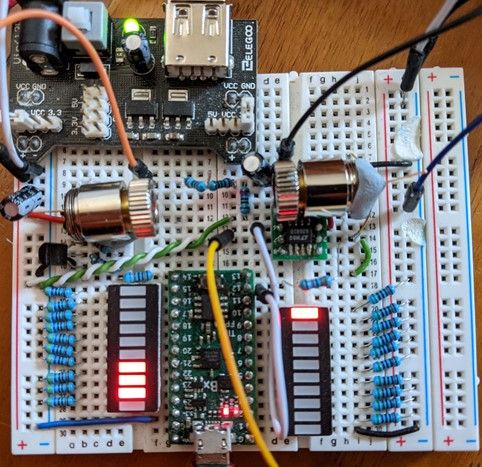
\includegraphics[width=\linewidth]{fig 29.jpg}\par}
\caption{Photo of the test setup for a LFSC using 2 culminating lenses.}
\label{fig}
\end{figure}

Completing further tests at different angles with a similar test setup to the original test. This time, at a bit rate of 2.6 Mbps to get a better idea of how angle affects the BER of the system.

Other potential additions to the system could be clock and data recovery, If successful it could prove to be very useful and demonstrate a technology that can communicate without sharing a clock.

\section*{Acknowledgment}

Dr. Roger Giddings, thank you for your patient supervision and guidance.

\begin{thebibliography}{00}
\bibitem{b1} Abdulsalam Ghalib Alkholidi and Khaleel Saeed Altowij (November 26th 2014). “Free Space Optical Communications — Theory and Practices, Contemporary Issues in Wireless Communications”, Mutamed Khatib, IntechOpen, DOI: 10.5772/58884. Available from: https://www.intechopen.com/books/contemporary-issues-in-wireless-communications/free-space-optical-communications-theory-and-practices]
\bibitem{b2} P. Kulshreshtha and A. K. Garg, "Managing 5G Networks - A Review of FSO Challenges and Solutions," 2020 11th International Conference on Computing, Communication and Networking Technologies (ICCCNT), Kharagpur, India, 2020, pp. 1-4, doi: 10.1109/ICCCNT49239.2020.9225591.
\bibitem{b3} M. S. Awan, Marzuki, E. Leitgeb, F. Nadeem, M. S. Khan and C. Capsoni, "Weather Effects Impact on the Optical Pulse Propagation in Free Space," VTC Spring 2009 - IEEE 69th Vehicular Technology Conference, Barcelona, 2009, pp. 1-5, doi: 10.1109/VETECS.2009.5073909.
\bibitem{b4} Polybius (1889). "Book X". The Histories of Polybius. pp. 43–46
\bibitem{b5} Bell, Alexander Graham. “The Photophone.” Science, vol. 1, no. 11, 1880, pp. 130–134. JSTOR, www.jstor.org/stable/2900889. Accessed 5 Dec. 2020.
\bibitem{b6} Boroson, D.M., Robinson, B.S. The Lunar Laser Communication Demonstration: NASA’s First Step Toward Very High Data Rate Support of Science and Exploration Missions. Space Sci Rev 185, 115–128 (2014). https://doi-org.ezproxy.bangor.ac.uk/10.1007/s11214-014-0122-y
\bibitem{b7} M. Toyoshima, "Recent Trends in Space Laser Communications for Small Satellites and Constellations," in Journal of Lightwave Technology, vol. 39, no. 3, pp. 693-699, 1 Feb.1, 2021, doi: 10.1109/JLT.2020.3009505.
\bibitem{b8} Suen, J.Y. Terabit-per-Second Satellite Links: a Path Toward Ubiquitous Terahertz Communication. J Infrared Milli Terahz Waves 37, 615–639 (2016). https://doi-org.ezproxy.bangor.ac.uk/10.1007/s10762-016-0257-x
\bibitem{b9} Arun Prakash, S., Sumithra, M.G., Shankar, K. et al. Performance investigation of spectral-efficient high-speed inter-satellite optical wireless communication link incorporating polarisation division multiplexing. Opt Quant Electron 53, 270 (2021). https://doi.org/10.1007/s11082-021-02950-8
\bibitem{b10} Ivannikov, V. & Kamkin, Alexander & Kossatchev, Alexander & Kuliamin, Victor & Petrenko, Alexander. (2007). The use of contract specifications for representing requirements and for functional testing of hardware models. Programming and Computer Software. 33. 272-282. 10.1134/S0361768807050039.
\bibitem{b11} (Basic Book/Monograph Online Sources) unknown. (1999). “Choosing a Collimation Lens for Your Laser Diode”. Unknown [online tutorial]. Volume(n/a). Available:https://www.thorlabs.com/newgrouppage9.cfm?objectgroup\_id=8790
\bibitem{b12} (Basic Book/Monograph Online Sources) unknown (2006, 05, 01). Laser radiation: safety advice [government website]. Volume (2). Available: http://www.(URLhttps://www.gov.uk/government/publications/laser-radiation-safety-advice/laser-radiation-safety-advice
\end{thebibliography}

\section{Appendix}
\subsection{16-bit LFSP Verilog code}

%Importing code from file
\lstinputlisting{A1.m}
\thispagestyle{empty} 
\pagenumbering{gobble}

\subsection{32-bit LFSP Verilog code}

%Importing code from file
\lstinputlisting{A2.m}
\subsection{The final Verilog code used in tests }

%Importing code from file
\lstinputlisting{A3.m}
\clearpage


\end{document}
